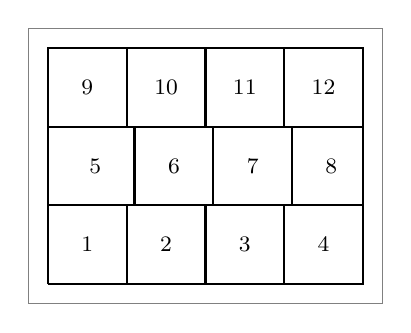
\begin{tikzpicture}
	\def \len{1}
	\def \eps{0.1}
	\def \del{0.25}
	\draw[thin, gray] (-\del, -\del) -- (-\del, 3*\len+\del) -- (4*\len+\del, 3*\len+\del) -- (4*\len+\del, -\del) -- (-\del, -\del);
	\draw[thick] (0, 0) -- (0, 3*\len) -- (4*\len, 3*\len) -- (4*\len, 0) -- (0, 0);	
	\draw[thick] (0, \len) -- (4*\len, \len);
	\draw[thick] (0, 2*\len) -- (4*\len, 2*\len);
	\foreach \x in {1,...,3}
	{ \draw[thick] (\x*\len, 0) -- (\x*\len, \len);
	  \draw[thick] (\x*\len+\eps, \len) -- (\x*\len+\eps, 2*\len);
	  \draw[thick] (\x*\len, 2*\len) -- (\x*\len, 3*\len);
	}
	\foreach \x in {0,...,11}
	{
	  	\pgfmathparse{int(floor(\x/4))};
  		\let\row\pgfmathresult
  		\pgfmathparse{int(\x - 4*\row)};
  		\let\col\pgfmathresult
  		\pgfmathparse{int(\x + 1)};
  		\let\y\pgfmathresult
  		\pgfmathparse{int(\row - 2*floor(\row/2))};
  		\let\rem\pgfmathresult
		\node[] at ({(\col + 0.5)*\len + \rem*\eps}, {(\row + 0.5)*\len}) {\footnotesize\y};
	}
\end{tikzpicture}